\chapter{System Implementation}

This chapter details the system implementation for the project.
Section~\ref{sec:im:arch} covers the implemented system architecture, while
Section~\ref{sec:im:code} details the implemented code base for the integrated
system. Finally, Section~\ref{sec:im:summ} summarises the contributions
made by the author in implementing the project.

The implementation shall satisfy all the requirements laid out in
Section~\ref{sec:in:obj}.

The source code for the system has been uploaded to GitHub~\cite{gh-magor};
GitHub also serves as the version control and issue management
system for the project~\cite{gh-magor-is}.

\section{System Architecture}\label{sec:im:arch}

This section describes the system architecture to realise the processing
pipelines. However before that, let us define some terminology specific
to our processing framework:

\begin{itemize}
    \item A \textit{module} is a self-contained piece of software to realise
    one component of a processing pipeline. Different modules are specified
    by unique \texttt{module\_id}'s.
    \item A \textit{procedure} is a collection of modules to realise a
    processing pipeline; it is defined by the modules and the order in which
    they are run. Different procedures are specified by unique
    \texttt{procedure\_id}'s; they might have overlapping modules depending
    on procedure design.
    \item A \textit{process} is a specific configuration of procedures; in
    different processes the specific procedure's modules could have different
    versions. The processes provide the basic version mechanism to satisfy
    the requirements in Section~\ref{sec:in:obj}; different processes are
    specified by unique \texttt{process\_id}'s.
\end{itemize}

With that, we define our system architecture of the following four components:

\begin{itemize}
    \item \textit{Data} --- the source and generated files from the various
    processing pipelines
    \item \textit{Modules} --- the core processing functionalities
    \item \textit{Manifests} --- the specific system configurations
    \item \textit{System Executable} --- the executable linking data and
    modules; runs according to the manifests and generating module calls on
    data
\end{itemize}

Figure~\ref{top-arch} describes the high-level description of the interaction
between these four components, and figure~\ref{top-lvl} provides the top-level
folder structure of the system.

\begin{figure}[ht]
\begin{center}
    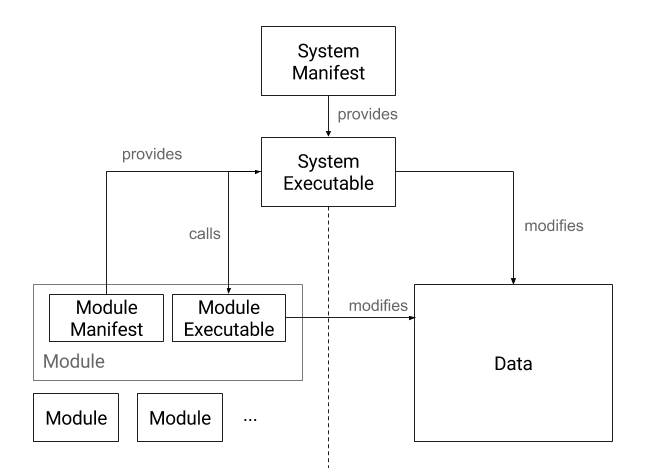
\includegraphics[width=0.9\textwidth]{system}
    \caption{High-level system architecture}\label{top-arch}
\end{center}
\end{figure}

\begin{figure}[ht]
\begin{lstlisting}
    crawl/
        --raw files--
    data/
        --data files--
    modules/
        --module files--
    system.py               # system executable
    manifest.json           # system manifest
\end{lstlisting}
\caption{Top-level folder structure}\label{top-lvl}
\end{figure}

The whole system would be implemented in Python, using JSON as the manifest
format owing to its inclusion in the Python standard library. The four
components would be described in detail in the following subsections.

\subsection{Data}\label{sec:im:arch:data}

The data used in the system are of two types. The first type is raw data, 
which are unprocessed audio or video files; these files are stored under
\texttt{crawl/}. The second type is processed data, which are stored under
\texttt{data/} in a specialised folder structure specified in Figure~\ref{data}:

\begin{figure}[ht]
\begin{lstlisting}
    data/
        process_id/
            file_id/
                raw/
                    --the raw file--
                module_1/
                    --output for module 1--
                module_2/
                    --output for module 2--
                ...
                module_n/
                    --output for module n--
                temp/
                    module_1/
                        --temporary files for module 1--
                    ...
\end{lstlisting}   
\caption{Data folder structure}\label{data} 
\end{figure}

Under this folder structure, the data is defined at the process and file level;
for each operation, the working folder (\texttt{working\_dir}) is set at
\texttt{data/process\_id/file\_id}, where \texttt{file\_id} denotes a unique
file identifier. This working folder would store all files associated with all
the modules in the respective process' procedures.

The data cycle could be seen as follows:

\begin{itemize}
    \item At system startup the system executable imports the raw file from
    \texttt{crawl/} into the \texttt{working\_dir/raw/} subfolder
    \item As a procedure is being executed, individual module's output files
    would be stored in the respective subfolder under \texttt{working\_dir},
    \item while the module's temporary files would be stored under
    \texttt{working\_dir/temp}
\end{itemize}

This structure allows the system to be fully modular; any module would only need
to know its own folder to dump íts output, and practically any operation could
be traced to the module level. Individual modules would be responsible in
implementing this structure.

\subsection{Modules}\label{sec:im:arch:mod}

All modules in the system are placed under the subfolder \texttt{modules/}
according to the folder structure described in Figure.
Each module has its own folder; the folder name is a module identifier in
the form of \texttt{module\_name-version}. This allows multiple versions of
a module to co-exist in the system. In each module folder there are three
compulsory components --- a \texttt{setup} script to setup the module and all
its dependencies, a Python executable \texttt{module.py} to call the module,
and a manifest file\footnote{The structure of this file would be detailed later
in the section on Manifests.} in JSON format to specify the module details.
The module setup script and executable could be run independently of the system
for development and testing purposes; this also ensures self-containment of the
module.

\begin{figure}[ht]
\begin{lstlisting}
    modules/
        module_id_1/
            setup           # module setup script
            module.py       # module executable
            manifest.json   # module manifest
            --optional module data and executables--
        module_id_2/
            ...
        ...            
\end{lstlisting}
\caption{Module folder structure}\label{module}
\end{figure}

\subsection{Manifests}\label{sec:im:arch:man}

There are two types of manifest in the implemented system --- modular manifest
and system manifest. Both types provide configuration options that are not
hard-coded into the system, allowing easy maintenance and upgrade.

\subsubsection{Modular manifests}

Each module has its own manifest, at the path \texttt{module\_id/manifest.json}
as specified in Figure~\ref{module}. The manifest file must conform to the
JSON structure specified in Figure~\ref{manifest-md}.

\begin{figure}[ht]
\begin{lstlisting}
    {
        "name": "module_name",
        "version": "module_version",
        "requires": [],
        "inputs": [],
        "outputs": []
    }
\end{lstlisting}
\caption{Modular manifest structure}\label{manifest-md}
\end{figure}

\texttt{requires}, \texttt{inputs} and \texttt{outputs} are all JSON lists.
\texttt{requires} is a list of (optional) data files and executables required
for the module's functionality; these files should be in place after running
the \texttt{setup} script. \texttt{inputs} and \texttt{outputs} are lists of
subfolders under \texttt{working\_dir}\footnote{See Section~\ref{sec:im:arch:data}
on Data.} where the module would pull its input files and push its output
files, respectively.

In this way, the manifest file serves as a blueprint of the module to the
system; this blueprint would be realised by the module executable.

\subsubsection{System manifest}

The system manifest specifies system-level properties; specifically the
processes, procedures and the file formats accepted by the system. It follows
the structure described in Figure~\ref{manifest-sys}; the fields' properties
are described in Table~\ref{table:manifest-sys}.

\begin{figure}[ht]
\begin{lstlisting}
    {
        "processes": {
            "process_id_1":{
                "module_id_1": "version",
                "module_id_2": "version",
                ...
            },
            ...
        }
        "default_process": "process_id",
        "procedures": {
            "procedure_id_1": [
                "module_name_1",
                "module_name_2",
                ...
            ],
            ...
        },
        "default_procedures": [],
        "file_types": {
            "audio": [],
            "video": []
        }
    }
\end{lstlisting}
\caption{System manifest structure}\label{manifest-sys}
\end{figure}

\begin{longtabu}{X[1.5,l]X[3.5,l]X[1,l]}
    \textbf{Field} & \textbf{Description} & \textbf{Type} \\
    \midrule
    \endhead{}
    \texttt{processes} &
    The processes in the system, specified by the module versions &
    \texttt{dict} \\
    \texttt{default\_process} &
    The default \texttt{process\_id} (if no process is specified to run,
    this process would be executed) &
    \texttt{str} \\
    \texttt{procedures} &
    The procedures in the system, specified by a list of module names &
    \texttt{dict} \\
    \texttt{default\_procedures} &
    The default \texttt{procedure\_id}'s (if no procedure is specified to
    run, these procedures would be executed) &
    \texttt{list\,(str)} \\
    \texttt{file\_types} &
    The file extensions accepted by the system &
    \texttt{dict} \\
    \caption{System manifest fields}\label{table:manifest-sys}
\end{longtabu}

In this way, the system manifest provides a blueprint of the whole system
to the system executable.

\subsection{System Executable}\label{sec:im:arch:sys-exec}

The system executable links the modules and data together by issuing module
calls on the data, given the manifest. A system run would proceed as follows:

\begin{itemize}
    \item Startup manifest checks --- load all manifests, perform error
    checks and eliminate invalid manifest items
    \item File import --- import the correct files from \texttt{crawl/}
    into the data structure in
    \texttt{data/}\footnote{See Section~\ref{sec:im:arch:data} on Data.}
    \item Pipeline --- call the modules in the procedure one-by-one in
    the order specified by the system manifest
\end{itemize}

\subsection{Evaluation of System Architecture}

The current system architecture described is able to satisfy three out of
five qualitative requirements outlined in Section~\ref{sec:in:obj}:

\begin{itemize}
    \item Modularity --- the well-defined components are independent and
    exhibits low coupling
    \item Extensibility --- the use of manifests allows for easy extension
    of system; components could be added independently of existing
    components and the system executable
    \item Versioning --- explicit versioning through the use of processes
    and different working folders per process
\end{itemize}

The next section would detail the code base implemented for the project,
which would address the primary objectives and the remaining qualitative
requirements.

\section{Implemented Code Base}\label{sec:im:code}

This section details the implemented Python codes for all the components
in the system. We would start with the system executable in
Section~\ref{sec:im:code:sys}. Then, each of the following four subsections
would detail the modules implemented for each of the four primary
objectives in Section~\ref{sec:in:obj} ---
Section~\ref{sec:im:code:trans} for single audio/video transcription,
Section~\ref{sec:im:code:mctr} for multi-channel recording transcription,
Section~\ref{sec:im:code:cap} for keyframe captioning and
Section~\ref{sec:im:code:viz} for visualization of transcripts and captions.
Thereafter, Section~\ref{sec:im:code:log} would briefly outline the system's
approach to logging; finally Section~\ref{sec:im:code:log} would summarise 
the entire implemented code base.

\subsection{System Executable}\label{sec:im:code:sys}

As described in Section~\ref{sec:im:arch:sys-exec}, the system executable
does three operations in a normal run --- manifest checks, file import and
processing pipeline. These operations would be encapsulated in two classes
\texttt{Manifest} and \texttt{Operation}. The CLI used to call the system
executable would be implemented using Python's \texttt{argparse} interface.

\subsubsection{Class \texttt{Manifest}}

This class holds the system and modular manifests\footnote{See
Section~\ref{sec:im:arch:man} on Manifests.}. Only one instance of the
class should be present every run.

The class constructor is aware of the location of system and modular
manifests, and would attempt to load the manifests into the following
instance attributes:

\begin{longtabu}{X[1,l]X[3,l]}
    \textbf{Attribute} & \textbf{Description} \\
    \midrule
    \endhead{}
    \texttt{processes} &
    The processes in system manifest \\
    \texttt{procedures} &
    The procedures in system manifest \\
    \texttt{def\_process} &
    The default process in system manifest \\
    \texttt{def\_procedures} &
    The default procedures in system manifest \\
    \texttt{valid\_types} &
    The valid file types in system manifest \\
    \texttt{modules} & 
    Modular manifests \\
    \caption{Attributes for class \texttt{Manifest}}
\end{longtabu}

The class provides three instance methods:

\begin{itemize}
    \item \texttt{check\_modules} to check the modular manifests, mainly
    for module requirements. Invalid modules would be removed from manifest.
    \item \texttt{check\_processes} to check the processes and procedures
    for inconsistencies in process definitions, procedure definitions and
    module versions. Invalid procedures and processes would also be removed
    from manifest.
    \item \texttt{check\_all} to wrap the two above-mentioned checks in
    the recommended order --- \texttt{check\_modules} followed by
    \texttt{check\_processes}
\end{itemize}

\subsubsection{Class \texttt{Operation}}

This class holds the definition for a single system ``operation''. An
operation is defined as a process' procedure applied on one file object;
usually there are more than one operation in a system run. The class
constructor is aware of the data structure\footnote{See
Section~\ref{sec:im:arch:data} on Data.}, and would attempt to initialize
the following instance attributes:

\begin{longtabu}{X[1,l]X[3,l]}
    \textbf{Attribute} & \textbf{Description} \\
    \midrule
    \endhead{}
    \texttt{file\_name} &
    The full name of the file in \texttt{crawl/} \\
    \texttt{file\_id} &
    The \texttt{file\_id} of the file object, used in determining
    the working folder \\
    \texttt{manifest} &
    The instance of class \texttt{Manifest} applicable \\
    \texttt{process\_id} &
    The \texttt{process\_id} of the process to be applied to the
    file object, used in determining the working folder \\
    \texttt{procedure\_id} &
    The \texttt{procedure\_id} of the procedure to be applied to the
    file object \\
    \texttt{working\_dir} & 
    The full path to the working directory \\
    \caption{Attributes for class \texttt{Operation}}
\end{longtabu}

The class provides four main instance methods:

\begin{itemize}
    \item \texttt{verify} to verify the operation against the checked
    manifest; set the module list if the method returns \texttt{True}
    \item \texttt{import\_file} to import raw files from \texttt{crawl/}
    to \texttt{working\_dir}
    \item \texttt{call} to call a single module executable on the
    \texttt{working\_dir}, using Python's \texttt{subprocess}. This call
    is atomic, since all modules follow the same structure\footnote{See
    Section~\ref{sec:im:arch:mod} on Modules.}
    \item \texttt{pipeline} to wrap the three above methods in a logical
    order --- \texttt{verify} first, if \texttt{True} does
    \texttt{import\_file} and repeatedly \texttt{call} on the modules
    in the module list, else throw an error and returns nothing. 
\end{itemize}

\subsubsection{System CLI}

The main system operations are encapsulated in two system functions,
\texttt{setup} and \texttt{process}. These two functions are attached
to two commands \texttt{setup} and \texttt{process} respectively
using \texttt{argparse}, as shown in Figure~\ref{args}.

\begin{figure}[ht]
\begin{lstlisting}
$ python system.py setup -h
usage: system.py setup [-h] [-m [module_id [module_id ...]]] [-a]

optional arguments:
    -h, --help            show this help message and exit
    -m [module_id [module_id ...]], --modules [module_id [module_id ...]]
                        module_ids to setup
    -a, --all             setup all available modules

$ python system.py process -h
usage: system.py process [-h] [-p [procedure_id [procedure_id ...]]]
                            [-f [file_name [file_name ...]]]
                            [-i [file_id [file_id ...]]] [-t] [-n]
                            [process_id]

positional arguments:
    process_id            process_id for this run

optional arguments:
    -h, --help            show this help message and exit
    -p [procedure_id [procedure_id ...]], --procedures [procedure_id [procedure_id ...]]
                        procedures to run
    -f [file_name [file_name ...]], --files [file_name [file_name ...]]
                        file_names to process
    -i [file_id [file_id ...]], --ids [file_id [file_id ...]]
                        file_ids to process
    -t, --test            just do system checks and exit
    -n, --simulate        simulate the run, without processing any file
\end{lstlisting}
\caption{System CLI}\label{args}
\end{figure}

\subsection{Modules for Transcription}\label{sec:im:code:trans}

As discussed in Section~\ref{sec:lr:trans}, we require three components
to realise the transcription pipeline in Figure~\ref{trans} --- a resampler,
a diarizer and a transcription engine. We would describe each component in
detail.

\subsubsection{Resampler (FFmpeg)}

The module \texttt{resample-1.0} is implemented using FFmpeg, through a
Python wrapper \texttt{FFmpy}~\cite{ffmpy}.

The module would take the raw file (either audio or video) from
\texttt{working\_dir/raw}, and resample it into an audio stream of the
following specification: single-channel WAVE file (\texttt{.wav}),
16000Hz sample rate and 16 bits per sample\footnote{The specification
is one used in all following components of the transcription pipeline.}.
The resampled file would be put into \texttt{working\_dir/resample}.

The setup script set up FFmpeg and \texttt{FFmpy} if they are not already in
the system. Complete checks are built into the module; if the resampled file
already exists, or if the raw file already has the correct specification, the
module is effectively a no-op.

\subsubsection{Diarization (LIUM)}

The module \texttt{diarize-8.4.1} is implemented using LIUM Speaker
Diarization version 8.4.1; Python's \texttt{subprocess} is used to interface
with LIUM's Java-based CLI\@.

The module would take the resampled \texttt{.wav} file from
\texttt{working\_dir/resample} and produce the segmentation file
(\texttt{.seg}) into \texttt{working\_dir/diarization}. The setup script
attempts to detect the installed Java version on the system; if Java is
not present or the version is earlier than Java 7, the script would
install the latest Java version (in this case Java 8) on the system.

Complete checks are built into the module; if the segmentation file
already exists, the module is effectively a no-op.

\subsubsection{Transcription Engine (Google Cloud Speech API)}

The module \texttt{google-1} is implemented using Cloud Speech API's
Python client library~\cite{gh-gcs}.

As the API is not free and rate-limited~\cite{gcs-free}, temporary files
would be used to store intermediate transcriptions offline. The engine
implementation is split into a four-stage pipeline described in
Figure~\ref{google}. Each stage is a function in the module; each function
would utilise a temporary file handler to look for temporary files
associated with that function. If the temporary files exist, the function
is determined to have been previously completed and acts as a no-op;
otherwise it would be executed as usual. The temporary file structure is
flexible enough to enable complete checks and resume at a segment level.

\begin{figure}[ht]
\begin{center}
    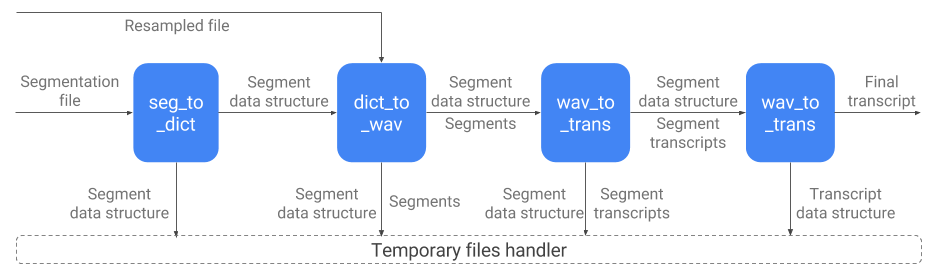
\includegraphics[width=0.9\textwidth]{pipeline_google}
    \caption{Module \texttt{google-1}}\label{google}
\end{center}
\end{figure}

Overall, the module would take the resampled file in
\texttt{working\_dir/resample} and the segmentation file in
\texttt{working\_dir/diarization}, and produce transcripts in both
plain \texttt{.txt} and Praat \texttt{.TextGrid} format~\cite{praat}
into \texttt{working\_dir/transcript/google}.
Temporary files would be stored in \texttt{working\_dir/temp/google}.
The setup script would install the Cloud Speech API client library and
remind developers to get a Google Service Account key to use the
Cloud Speech API~\cite{gcs-api-key}.

\subsubsection{Transcription Engine (Kaldi)}

The module \texttt{lvcsr-1701} is implemented using the Kaldi 
scripts and models provided by Dr.\ Xu Haihua of SLRG\@. The models
are trained to recognize English on a dataset of Singaporean audio and
video files, for evaluation against a ``black box'' toolkit such as
Google Cloud Speech API\@.

As the scripts are all batched, a Python wrapper using \texttt{subprocess}
is developed. The files (and temporary files) are re-directed, such that
the module could take the resampled file from \texttt{working\_dir/resample}
and the segmentation file in \texttt{working\_dir/\\diarization}, and produce
transcripts in various formats, including Praat \texttt{TextGrid} into
\texttt{working\_dir/transcript/lvcsr}. The temporary files would be stored
in \texttt{working\\ \_dir/temp/lvcsr}.

The setup script would attempt to detect an installation of Kaldi in the
system; if no such installation is found, the script would download and
build Kaldi in a specific location under the user's \texttt{/home/} folder.
The script would also download the LVCSR models of Dr.\ Xu Haihua\footnote{
This would only work if the user has access to SLRG's resources, as the
models are behind SLRG's cluster servers.}.

\subsection{Modules for Multi-channel Recording
Transcription}\label{sec:im:code:mctr}

As discussed in Section~\ref{sec:lr:trans}, multi-channel recording VAD
is required before transcription is performed. Furthermore, as there would
be multiple files involved in a multi-channel recording, modules that only
take one input file in Section~\ref{sec:im:code:trans} must be adapted to
process multiple files.

\subsubsection{Reconfiguring resampler for multi-channel recording}

The module \texttt{resample-1.0} initially only takes in one raw file from
\texttt{working\_dir/raw}. To enable multi-channel capabilities, a switch is
added on the count of (valid) files in \texttt{working\_dir/raw}: if it's 1,
then follow the single file pipeline, else resample the files one-by-one and
put the resampled files into \texttt{working\_dir/resample}\footnote{A
switch is necessary even though the output folder is still the same, because
the file name behaviours are different.}.

\subsubsection{Multi-channel VAD}

The module \texttt{vad-1.0} is implemented using the Python codebase of
Prof.\ Chng Eng Siong and Mr.\ Pham Van Tung of SLRG\@. A wrapper function
is added to the existing codebase, enabling the codebase to take in resampled
inputs from \texttt{working\_dir/\\resample} and produce the VAD output
(clean speech-segmentation file pairs) into \texttt{working\_dir/vad}.
The temporary files are stored in \texttt{working\_dir/temp/vad}.

As the Python codebase depends on a few libraries such as \texttt{numpy},
\texttt{scipy} and \texttt{soundfile}, the setup script would install
those libraries.

\subsubsection{Reconfiguring transcription engine (Google Cloud Speech API)
for multi-channel recording}

The module \texttt{google-1} initially takes in one resampled file from
\texttt{working\_dir/resample} and one segmentation file from
\texttt{working\_dir/diarization}. However, for multi-channel recordings,
the VAD outputs are in pairs in \texttt{working\_dir/vad}. A switch is
added on the existence of files in \texttt{working\_dir/diarization}:
if there is exactly one, it defaults to the single-file scenario;
else the module would iterate through all clean speech-segmentation file
pairs in \texttt{working\_dir/vad}, treating each pair as one ``resampled''
file and one ``segmentation'' file and apply the same output and temporary
folders.

\subsection{Modules for Keyframe Captioning}\label{sec:im:code:cap}

As discussed in Section~\ref{sec:lr:cap}, two components are necessary
to realise the captioning pipeline in Figure~\ref{cap} --- a video
converter and a caption generator. The implementation of the two
components would be detailed below.

\subsubsection{Video converter (FFmpeg)}

The module \texttt{convert-1.0} is implemented using FFmpeg, through the
same Python wrapper \texttt{FFmpy}~\cite{ffmpy}.

The module would take the raw video file from \texttt{working\_dir/raw},
and convert it into an \texttt{.mp4} file, retaining all charateristics
of the raw video file\footnote{The specification is chosen because of
ubiquity.}. The converted file would be put into \texttt{working\_dir/convert}.

The setup script set up FFmpeg and \texttt{FFmpy} if they are not already in
the system. Complete checks are built into the module; if the converted file
already exists, or if the raw file is already in \texttt{.mp4}, the
module is effectively a no-op.

\subsubsection{Caption generator (NeuralTalk2)}

The module \texttt{capgen-1.0} is implemented using the Python codebase of
Peter~\cite{peter}, another Final-Year Project under SLRG\@. The codebase
utilises NeuralTalk2~\cite{gh-nrtalk2} and its pretrained model, so that
we do not have to train our own models to generate captions. Keyframes are
extracted using FFmpeg; a wrapper function is added into the codebase so
that the module could take in the converted video file from
\texttt{working\_dir/convert}, and generate keyframes and their caption
(in JSON format) into \texttt{working\_dir/capgen}.

In the initial codebase, complete checks are not fully implemented (the
caption generator would always run on all images). The temporary file
structure has been adapted; individual captions are saved into temporary as
they are created, allowing full and partial complete checks at all points
in the caption generation pipeline. The temporary files are stored in
\texttt{working\_dir/temp/capgen}.

As the codebase relies on Torch~\cite{th}, the setup script takes care
of Torch detection and installation. The script would also download the
necessary pre-trained models for NeuralTalk2.

\subsection{Modules for Visualization}\label{sec:im:code:viz}

The aim of visualization is to visually compared the different transcripts
and captions generated by the pipeline. Two visualizations are usually
prefered:

\begin{itemize}
    \item Praat's \texttt{TextGrid} format
    \item SubRip subtitles on video (\texttt{.srt})~\cite{srt}
\end{itemize}

As described in Section~\ref{sec:im:code:trans} and~\ref{sec:im:code:mctr},
the transcripion pipeline already produces transcript in \texttt{TextGrid}
format. However, to visualize these transcription the Praat software is
required; although Praat is widely used and very powerful, its interface is
hard to grasp at first glance. To enable quick, visual comparison of transcripts
and captions, the module \texttt{visualize-1.0} produces two items:

\begin{itemize}
    \item A video file in \texttt{.mp4}
    \item An accompanying subtitle (\texttt{.srt})
\end{itemize}

The video file could be opened in many video viewers, and accompanying subtitles
would load automatically. Since we are handling three different pipelines,
the way this module would handle each pipeline is different; however the
video and subtitle are always produced in \texttt{working\_dir/visualize}.
The steps are summarised in Table~\ref{viz}.

\begin{longtabu}{X[1,l]X[2,l]X[2,l]}
    \textbf{Pipeline} & \textbf{Video handling}
    & \textbf{Subtitle handling} \\
    \midrule
    \endhead{}
    Single-audio transcripion &
    Convert resampled audio to black-screen video &
    Convert \texttt{.TextGrid} into \texttt{.srt} \\
    Single-video transcription &
    Copy converted video &
    Convert \texttt{.TextGrid} into \texttt{.srt} \\
    Multi-channel recording transcription &
    Merge (clean) channels into audio, convert to black-screen video &
    Merge individual channel \texttt{.TextGrid}'s into \texttt{.srt} \\
    Keyframe captioning &
    Copy converted video &
    Convert JSON captions into \texttt{.srt} \\
    \caption{Visualization steps}\label{viz}
\end{longtabu}

The video handling is implemented using FFmpeg through the Python wrapper
\texttt{FFmpy}~\cite{ffmpy}. The setup script would take care of installing
FFmpeg and \texttt{FFmpy}.

\subsection{Logging}\label{sec:im:code:log}

Logging is implemented in the system through Python's standard
\texttt{logging} library, and is present on two levels.

\subsubsection{System Executable}

The \texttt{logging} header in Figure~\ref{log-sys} is presented in the
system executable.

\begin{figure}[ht]
\begin{lstlisting}
logging.basicConfig(level=logging.DEBUG,
                    format='%(asctime)s (%(name)s | %(levelname)s) : %(message)s')
LOG = logging.getLogger('system')
\end{lstlisting}
\caption{System executable logging header}\label{log-sys}
\end{figure}

This header sets the system default logging level to \texttt{DEBUG}, and prints
out logging message with time and the name of the logger (set to \texttt{'system'}).
Most behaviours in the two classes \texttt{Manifest} and \texttt{Operation} are
logged, with level \texttt{INFO}.

\subsubsection{Module}

The \texttt{logging} header in Figure~\ref{log-mod} is presented in all
module executable.

\begin{figure}[ht]
\begin{lstlisting}
MODULE_NAME = 'module_name'
LOG_H = logging.StreamHandler()
LOG_F = logging.Formatter(
    '%(asctime)s (%(name)s | %(levelname)s) : %(message)s')
LOG_H.setFormatter(LOG_F)
LOG = logging.getLogger(MODULE_NAME)
LOG.propagate = False
LOG.addHandler(LOG_H)
LOG.setLevel(logging.DEBUG)
\end{lstlisting}
\caption{Module executable logging header}\label{log-mod}
\end{figure}

This header sets the default modular logging level to \texttt{DEBUG}, and prints
out logging message with time and the name of the logger (set to the module name).
The modular logger thread is independent of the system logger thread, although
the message format is the same; modular behaviours are logged with level
\texttt{DEBUG}.

\subsection{Summary}\label{sec:im:code:summ}

The current system implementation described is able to satisfy all primary
objectives in Section~\ref{sec:in:obj}; four pipelines are developed respectively
to address individual primary objective. Additionally, it satisfies three out of
five qualitative requirements outlined in Section~\ref{sec:in:obj}:

\begin{itemize}
    \item Extensibility --- the conversion from single audio/video transcription
    to multi-channel recording transcription demonstrates the ease of extending
    the system to a new scenario
    \item Robustness --- there is robust error checking, recovery, complete checks
    and resumes at the modular level
    \item Logging --- there is adequate logging for developers and users'
    understanding of system operations and output
\end{itemize}

The next section summarises the whole implementation of our project.

\section{Summary of System Implementation}\label{sec:im:summ}

Section~\ref{sec:im:arch} and~\ref{sec:im:code} details the system architecture
and the implemented code base for the system, that satisfies all the requirements
in Section~\ref{sec:in:obj}.

The contributions of the author to the project is summarised in
Table~\ref{contribs}.

\begin{longtabu}{X[1,l]X[2,l]}
    \textbf{Component} & \textbf{Contributions} \\
    \midrule
    \endhead{}
    System architecture &
    Develop the system architecture (100\%) \\
    System executable &
    Develop the Python executable (100\%) \\
    Module \texttt{resample} &
    Develop the Python module and setup script (100\%) \\ 
    Module \texttt{diarize} & 
    Develop the Python wrapper around external module
    and setup script (100\%) \\
    Module \texttt{google} &
    Develop the Python module and setup script (100\%) \\
    Module \texttt{lvcsr} &
    Modify the existing module to fit the system
    requirements, develop the setup script (50\%)\\
    Module \texttt{vad} &
    Modify the existing module to fit the system
    requirements, develop the setup script (50\%)\\
    Module \texttt{convert} &
    Develop the Python module and setup script (100\%)\\
    Module \texttt{capgen} &
    Modify the existing module to fit the system
    requirements, develop the setup script (50\%)\\
    Module \texttt{visualize} &
    Develop the Python module and setup script (100\%) \\
    \caption{Summary of contributions}\label{contribs}
\end{longtabu}

The next chapter presents the evaluation of the system on test data.
